\documentclass[10pt]{beamer}

% --- Theme Setup ---
\usetheme{Madrid}
\usecolortheme{whale}
\usefonttheme{default}

% --- Packages ---
\usepackage[utf8,nocaptions]{vietnam}
\usepackage[vietnamese]{babel}
\usepackage{graphicx}
\usepackage{subcaption}
\usepackage{booktabs}
\usepackage{amsmath}
\usepackage{amsfonts}
\usepackage{array}
\usepackage{float}
\usepackage{url}

% --- Custom Colors (Sleek Dark Blue Theme) ---
\definecolor{deepblue}{RGB}{22,33,62}
\definecolor{midblue}{RGB}{15,76,129}
\setbeamercolor{structure}{fg=midblue}
\setbeamercolor{titlelike}{parent=structure,bg=deepblue,fg=white}

% --- Title Slide Info ---
\title[Ứng dụng mô hình LP cho Knapsack]{ỨNG DỤNG CÁC MÔ HÌNH QUY HOẠCH TUYẾN TÍNH \\ CHO CÁC LOẠI BÀI TOÁN KNAPSACK}
\subtitle{Báo cáo Tiểu luận môn học}
\author[Nguyễn H. Đạt, Lê S. Thức, Nguyễn H. Anh]{
    Nguyễn Hoàng Đạt - 24001989 \\
    Lê Sỹ Thức - 25000312 \\
    Nguyễn Hải Anh - 24001968
}
\institute[HUS]{
    Trường Đại học Khoa học Tự nhiên \\
    Đại học Quốc gia Hà Nội
}
\date[2026]{Hà Nội, 2026}

\begin{document}

% --- Slide 1: Title ---
\begin{frame}
    \titlepage
\end{frame}

% --- Slide 2: Đặt vấn đề ---
\begin{frame}{Đặt vấn đề \& Phát biểu bài toán}
    \begin{block}{Bài toán xếp ba lô (Knapsack Problem)}
        Chọn một tập hợp đồ vật có khối lượng $w_i$ và giá trị $v_i$ xếp vào ba lô sức chứa $W$ sao cho tổng giá trị lớn nhất.
    \end{block}
    \vspace{0.3em}
    \textbf{3 biến thể chính:}
    \begin{itemize}
        \item \textbf{0/1 Knapsack:} Mỗi đồ vật chỉ được chọn tối đa $1$ lần ($x_i \in \{0,1\}$). $\rightarrow$ \textbf{NP-khó (Karp, 1972)}.
        \item \textbf{Unbounded Knapsack:} Số lượng đồ vật chọn là không giới hạn ($x_i \in \mathbb{Z}^+$).
        \item \textbf{Fractional Knapsack:} Đồ vật có thể phân chia, cho phép chọn một phần ($x_i \in [0,1]$). $\rightarrow$ Giải được bằng đơn hình hoặc tham lam trong thời gian đa thức.
    \end{itemize}
\end{frame}

% --- Slide 3: Giải thuật cơ sở (Baselines) ---
\begin{frame}{Các giải thuật cơ sở làm hệ quy chiếu (Baselines)}
    \begin{columns}
        \begin{column}{0.5\textwidth}
            \textbf{1. Giải thuật xấp xỉ:}
            \begin{itemize}
                \item \texttt{GreedyFractional:} Sắp xếp theo tỷ số density $v_i / w_i$ và chọn tuần tự. Độ phức tạp $\mathcal{O}(n \log n)$.
            \end{itemize}
            \textbf{2. Giải thuật chính xác tổ hợp:}
            \begin{itemize}
                \item \texttt{Backtracking:} Duyệt toàn bộ cây nhị phân, độ phức tạp $\mathcal{O}(2^n)$.
                \item \texttt{BranchAndBound:} Cắt nhánh bằng cận trên Fractional relaxation rất chặt.
            \end{itemize}
        \end{column}
        \begin{column}{0.5\textwidth}
            \textbf{3. Quy hoạch động (DP):}
            \begin{itemize}
                \item Áp dụng công thức truy hồi dựa trên trạng thái con.
                \item Độ phức tạp thời gian và bộ nhớ: $\mathcal{O}(n \cdot W)$ (giả đa thức - pseudo-polynomial).
                \item \texttt{DPUnbounded} tối ưu hóa bộ nhớ xuống mảng 1 chiều kích thước $W$.
            \end{itemize}
        \end{column}
    \end{columns}
\end{frame}

% --- Slide 4: Quy hoạch tuyến tính & Đơn hình ---
\begin{frame}{Quy hoạch tuyến tính (LP Relaxation) \& Thuật toán Đơn hình}
    \begin{block}{Continuous Relaxation của 0/1 Knapsack}
        Nới lỏng điều kiện nguyên thành $0 \le x_i \le 1$. Bài toán được đưa về dạng mô hình LP tổng quát.
    \end{block}
    \vspace{0.3em}
    \textbf{Primal Simplex vs. Dual Simplex:}
    \begin{itemize}
        \item \textbf{Primal Simplex:} Duy trì tính khả thi gốc (primal feasibility) và cải thiện hàm mục tiêu qua các bước xoay pivot.
        \item \textbf{Dual Simplex:} Duy trì tính khả thi đối ngẫu (dual feasibility) và khôi phục tính khả thi gốc.
    \end{itemize}
    \begin{alertblock}{Đặc điểm của Dual Simplex}
        Rất phù hợp để giải quyết các bài toán relaxation khi chèn thêm ràng buộc mới (như trong Branch-and-Bound hay Gomory Cut). Không cần chạy Phase I từ đầu mà có thể \textbf{Warm-start} trực tiếp để tìm nghiệm tối ưu mới sau $1 \rightarrow 5$ bước xoay pivot.
    \end{alertblock}
\end{frame}

% --- Slide 5: Quy hoạch nguyên: Phương pháp Gomory Cut ---
\begin{frame}{Quy hoạch nguyên: Lát cắt Gomory (Gomory Cut)}
    \begin{block}{Cơ chế sinh lát cắt Gomory}
        Từ dòng tối ưu liên tục có biến cơ sở không nguyên $x_i^* = \bar{b}_i \notin \mathbb{Z}$:
        $$x_i + \sum_{j \in J} \bar{a}_{ij} x_j = \bar{b}_i$$
        Lát cắt Gomory (Gomory fractional cut) loại bỏ nghiệm không nguyên hiện tại:
        $$\sum_{j \in J} (\bar{a}_{ij} - \lfloor \bar{a}_{ij} \rfloor) x_j \ge \bar{b}_i - \lfloor \bar{b}_i \rfloor$$
    \end{block}
    \textbf{Thách thức hội tụ số học (Floating-point precision limits):}
    \begin{itemize}
        \item Trong Python thuần (số thực kép 64-bit IEEE 754), sai số làm tròn tích lũy qua các phép xoay pivot và khử Gauss dẫn đến tính toán phần lẻ bị lệch nhẹ.
        \item Gây ra các lát cắt bị nhiễu số học, dẫn đến hiện tượng **không hội tụ (cycling/infinite loop)** và làm tăng tỷ lệ timeout của Gomory Cut lên $86,3\%$.
    \end{itemize}
\end{frame}

% --- Slide 6: Quy hoạch nguyên: Simplex Branch-and-Bound ---
\begin{frame}{Simplex Branch-and-Bound (BnB)}
    \begin{itemize}
        \item \textbf{Nguyên lý:} Phân nhánh trên biến $x_i^* \notin \mathbb{Z}$ bằng cách chèn trực tiếp ràng buộc nhánh $x_i \le \lfloor x_i^* \rfloor$ và $x_i \ge \lceil x_i^* \rfloor$ vào bảng đơn hình hiện tại.
        \item \textbf{Tối ưu hóa:} Giải lại (Warm-start) bằng Dual Simplex cực nhanh.
    \end{itemize}
    \begin{block}{Điểm nghẽn tính toán (Gaussian Elimination)}
        Để tránh ma trận tableau phình to, thuật toán chạy khử Gauss $\mathcal{O}(m^2 n)$ để lọc bỏ các ràng buộc dư thừa ở mỗi nút.
        \begin{itemize}
            \item Ở quy mô $n = 750$, với $m \approx 750$ ràng buộc, số phép tính tại mỗi nút đạt xấp xỉ $750^2 \times 750 \approx 4,2 \times 10^8$ phép tính.
            \item Việc thực thi vòng lặp lồng lớn này bằng Python thuần (không JIT/C compiled) gây ra tỷ lệ timeout cao ($85,2\%$).
        \end{itemize}
    \end{block}
\end{frame}

% --- Slide 7: Thiết lập thực nghiệm ---
\begin{frame}{Thiết lập thực nghiệm}
    \begin{itemize}
        \item \textbf{Quy mô:} Tổng cộng 8.220 lượt chạy trên 822 testcase ngẫu nhiên.
        \item \textbf{4 Kịch bản kiểm thử:}
            \begin{itemize}
                \item \texttt{core\_exact}: $N \le 50$, kiểm tra thuật toán chính xác.
                \item \texttt{core\_heuristic}: $N \le 1000$, so sánh tiệm cận và khả năng chịu tải.
                \item \texttt{stress}: $W \approx 50.000$, thử thách thuật toán quy hoạch động.
                \item \texttt{extreme\_n\_test}: $N \le 10.000$, kiểm tra giới hạn của giải thuật tham lam.
            \end{itemize}
        \item \textbf{Môi trường:} Python 3.14, NumPy 2.x, SciPy 1.x. Đo lường cách ly tiến trình (Process Isolation) để khử nhiễu từ bộ thu gom rác (Garbage Collector).
    \end{itemize}
\end{frame}

% --- Slide 8: Kết quả thực nghiệm: Thời gian thực thi ---
\begin{frame}{Kết quả thực nghiệm: Phân phối trạng thái chạy}
    \begin{columns}
        \begin{column}{0.55\textwidth}
            \begin{figure}[H]
                \centering
                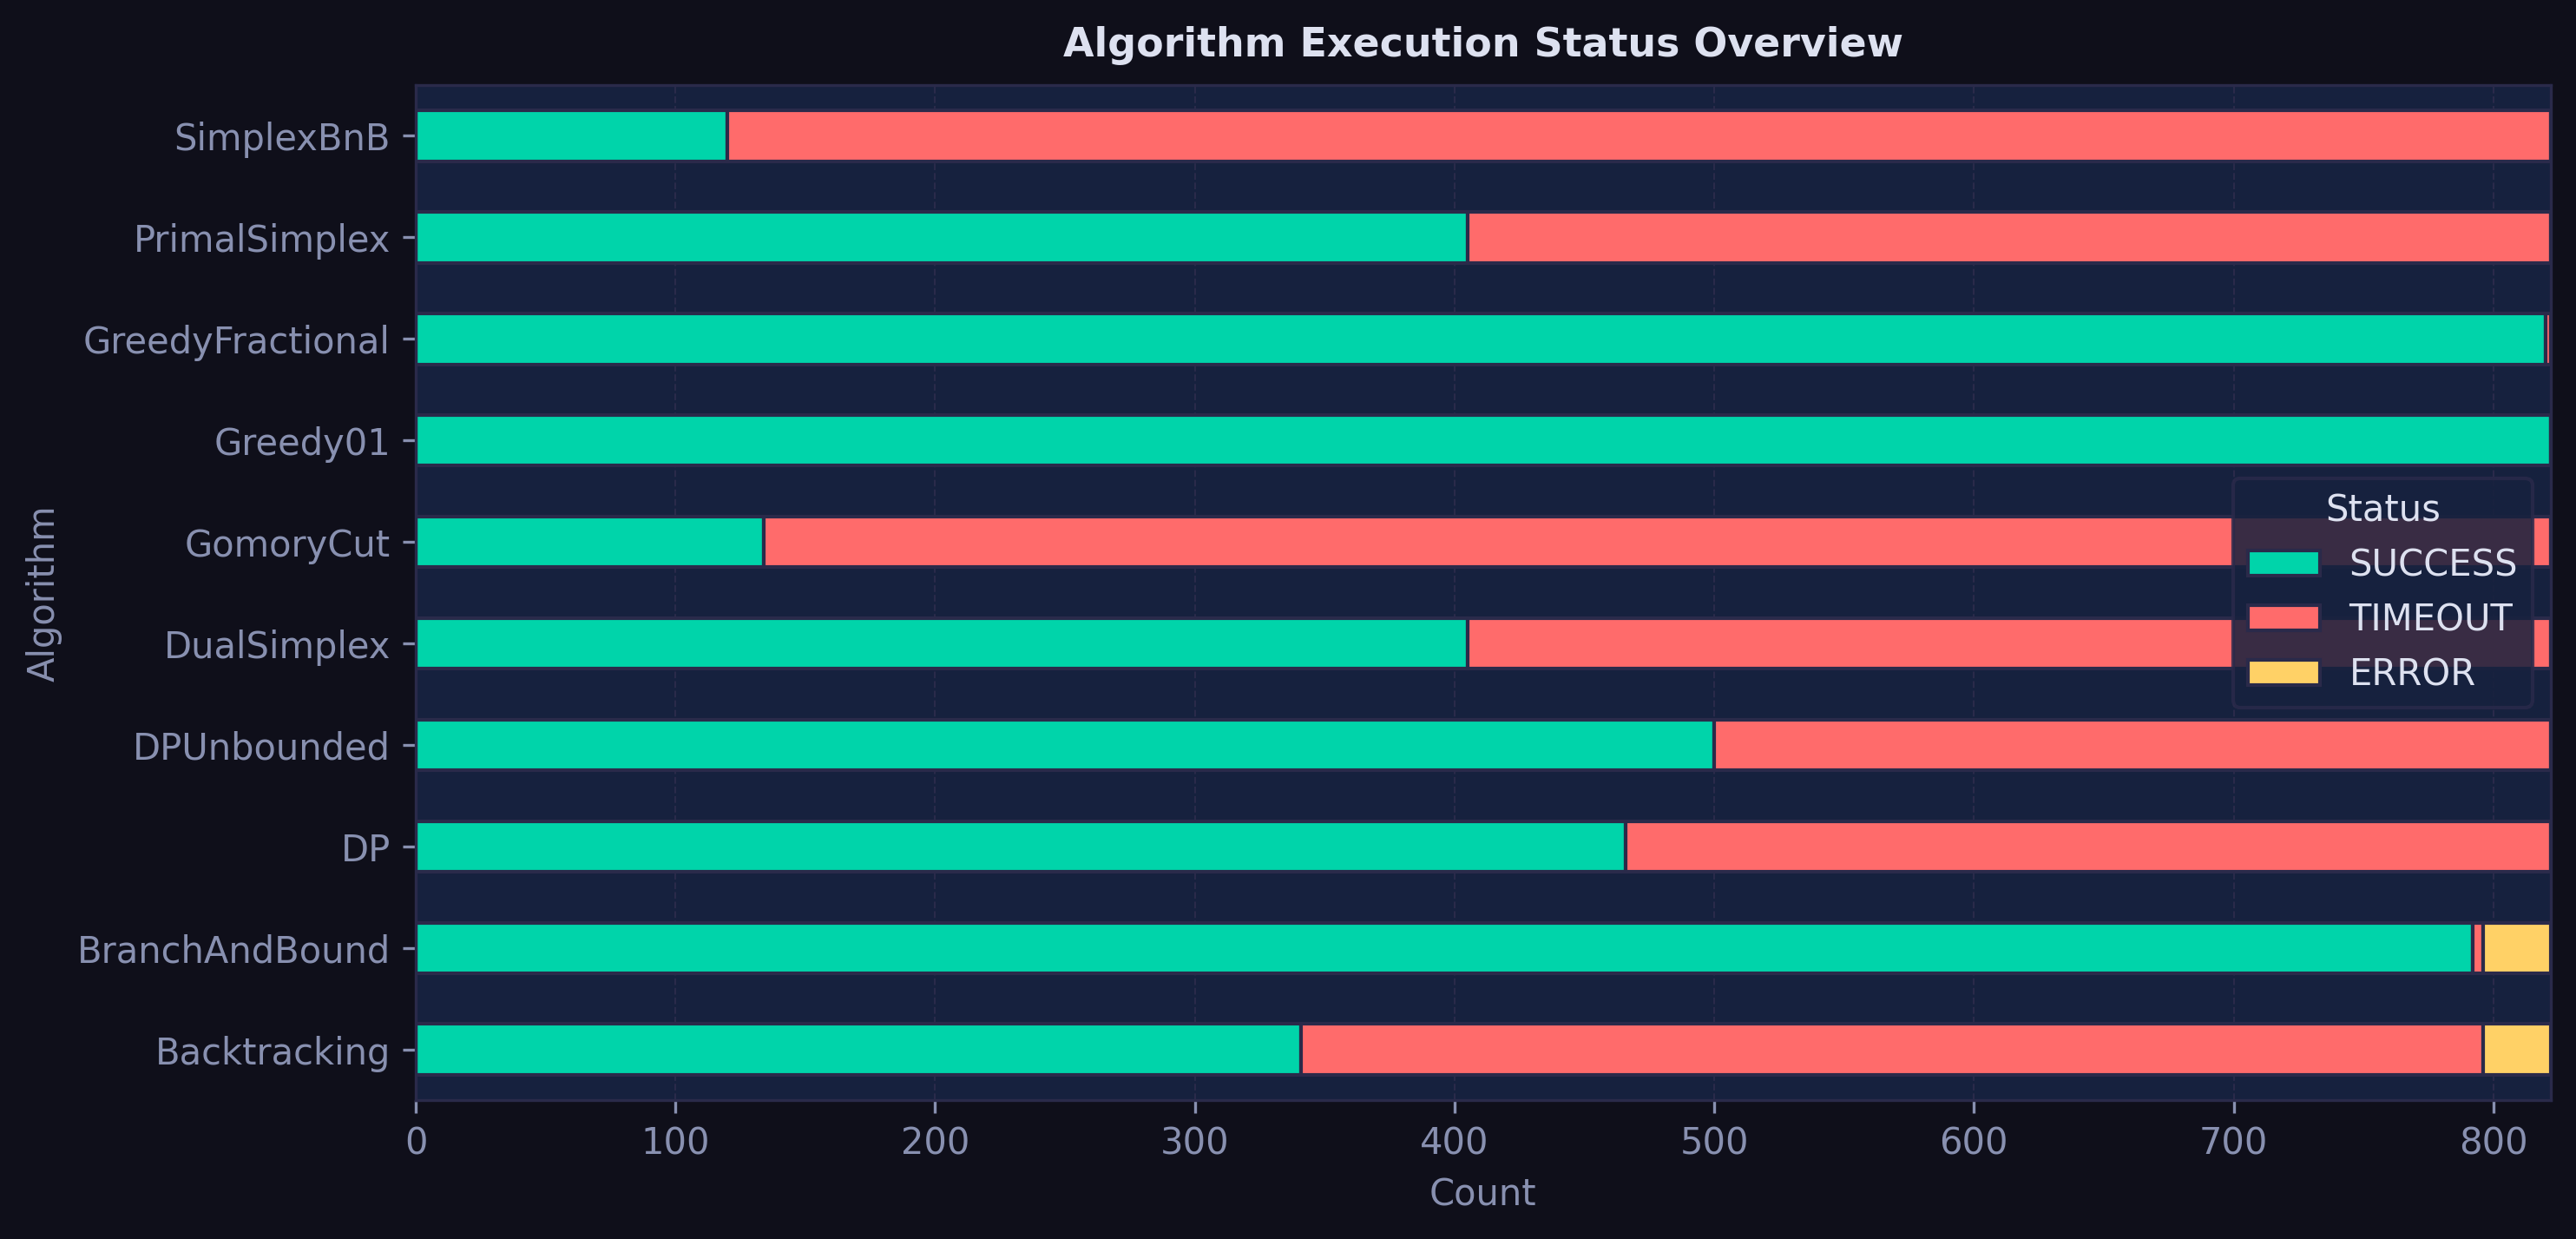
\includegraphics[width=\textwidth]{image/algo_status_comparison.png}
                \caption{Trạng thái chạy của 10 thuật toán.}
            \end{figure}
        \end{column}
        \begin{column}{0.45\textwidth}
            \small
            \textbf{Nhận xét từ Bảng số liệu SUCCESS:}
            \begin{itemize}
                \item \texttt{GreedyFractional} và \texttt{Greedy01}: Tốc độ cực nhanh (trung vị $< 0,2$\,ms), tỷ lệ thành công 100\%.
                \item \texttt{BranchAndBound} combinatorial: Hiệu năng xuất sắc (trung vị $1,65$\,ms, timeout $0,1\%$).
                \item \texttt{DualSimplex} và \texttt{PrimalSimplex}: Trung vị khoảng $189$\,ms.
                \item \texttt{SimplexBnB} và \texttt{GomoryCut}: Thời gian chạy trung bình lớn ($1,28$\,s và $0,65$\,s), timeout $> 85\%$.
            \end{itemize}
        \end{column}
    \end{columns}
\end{frame}

% --- Slide 9: So sánh thời gian thực thi theo kích thước $N$ ---
\begin{frame}{So sánh thời gian thực thi theo kích thước $N$}
    \begin{figure}[H]
        \centering
        
\includegraphics[width=0.85\textwidth]{image/runtime_comparison_fractional.png}
        \caption{So sánh thời gian chạy trong bài toán Fractional Knapsack (Greedy vs Simplex).}
    \end{figure}
    \begin{itemize}
        \item Sắp xếp tham lam \texttt{GreedyFractional} vượt trội hơn hẳn so với việc giải hệ phương trình đơn hình của Primal và Dual Simplex.
        \item Tuy nhiên, Simplex giải quyết được các bài toán ràng buộc tổng quát và cung cấp thông tin đối ngẫu.
    \end{itemize}
\end{frame}

% --- Slide 10: So sánh bộ nhớ sử dụng thực tế ---
\begin{frame}{So sánh bộ nhớ sử dụng thực tế}
    \begin{columns}
        \begin{column}{0.55\textwidth}
            \begin{figure}[H]
                \centering
                
\includegraphics[width=\textwidth]{image/memory_comparison.png}
                \caption{Phân phối bộ nhớ sử dụng của các thuật toán.}
            \end{figure}
        \end{column}
        \begin{column}{0.45\textwidth}
            \textbf{Ưu thế bộ nhớ của Simplex/ILP:}
            \begin{itemize}
                \item \textbf{DP truyền thống:} Yêu cầu bảng quy hoạch động kích thước $(n+1) \times (W+1)$, bộ nhớ bùng nổ theo cấp số nhân $\mathcal{O}(n W)$ lên tới **$88,8$\,MB**.
                \item \textbf{Simplex/ILP:} Chỉ sử dụng bảng Đơn hình (Tableau) kích thước $(m+1) \times (n+m+2)$ phần tử số thực. Bộ nhớ đỉnh luôn được khống chế dưới **$1$\,MB**, hoàn toàn độc lập với sức chứa túi $W$.
            \end{itemize}
        \end{column}
    \end{columns}
\end{frame}

% --- Slide 11: Khớp đường cong thực nghiệm (Curve Fitting) ---
\begin{frame}{Khớp đường cong thực nghiệm (Curve Fitting)}
    \begin{columns}
        \begin{column}{0.5\textwidth}
            \begin{figure}[H]
                \centering
                
\includegraphics[width=\textwidth]{image/curvefit/curvefit_DP.png}
                \caption{DP: Khớp Bậc ba, $R^2 = 0,79$.}
            \end{figure}
        \end{column}
        \begin{column}{0.5\textwidth}
            \begin{figure}[H]
                \centering
                
\includegraphics[width=\textwidth]{image/curvefit/curvefit_BranchAndBound.png}
                \caption{BranchAndBound: Khớp Bậc ba, $R^2 = 0,50$.}
            \end{figure}
        \end{column}
    \end{columns}
    \begin{block}{Khớp thực nghiệm số bước xoay pivot của Simplex}
        Trường hợp xấu nhất của Simplex là hàm mũ (khối Klee-Minty), nhưng thực tế trên bài toán Knapsack chỉ ra số bước xoay pivot tăng trưởng tuyến tính hoặc đa thức bậc cực thấp ($R^2 \ge 0,90$). Điều này chứng minh hiệu năng trung bình cực kỳ tốt của Đơn hình.
    \end{block}
\end{frame}

% --- Slide 12: Phân tích độ nhạy (Sensitivity Analysis) ---
\begin{frame}{Phân tích độ nhạy (Sensitivity Analysis)}
    \begin{block}{Mục tiêu}
        Đánh giá hiệu quả của cơ chế \textbf{Warm-start} (tận dụng cơ sở tối ưu cũ) bằng Đơn hình đối ngẫu khi các tham số của bài toán Knapsack bị biến động động, thay vì giải lại từ đầu (Re-solve).
    \end{block}
    \textbf{3 Kịch bản biến động tham số thực nghiệm (200 mẫu):}
    \begin{enumerate}
        \item \textbf{Thay đổi sức chứa ba lô W (Capacity RHS):} Tăng $W$ thêm $15\%$. Tọa độ nghiệm thay đổi $x_B = B^{-1}(b + \Delta b)$. Giữ nguyên tính đối ngẫu, áp dụng **Dual Simplex** để sửa tính khả thi gốc.
        \item \textbf{Thay đổi hệ số hàm mục tiêu c (Values):} Tăng giá trị $c_0$ thêm $25\%$. Giữ nguyên tính khả thi gốc, áp dụng **Primal Simplex** nếu mất tính tối ưu đối ngẫu.
        \item \textbf{Thêm ràng buộc phụ mới (Volume Constraint):} Thêm ràng buộc $\sum v_i x_i \le V_{max}$. Nghiệm cũ có thể vi phạm ràng buộc (biến bù âm), giải quyết nhanh bằng **Dual Simplex**.
    \end{enumerate}
\end{frame}

% --- Slide 13: Hiệu năng Warm-start bằng Đơn hình đối ngẫu ---
\begin{frame}{Hiệu năng Warm-start bằng Đơn hình đối ngẫu}
    \begin{columns}
        \begin{column}{0.5\textwidth}
            \begin{figure}[H]
                \centering
                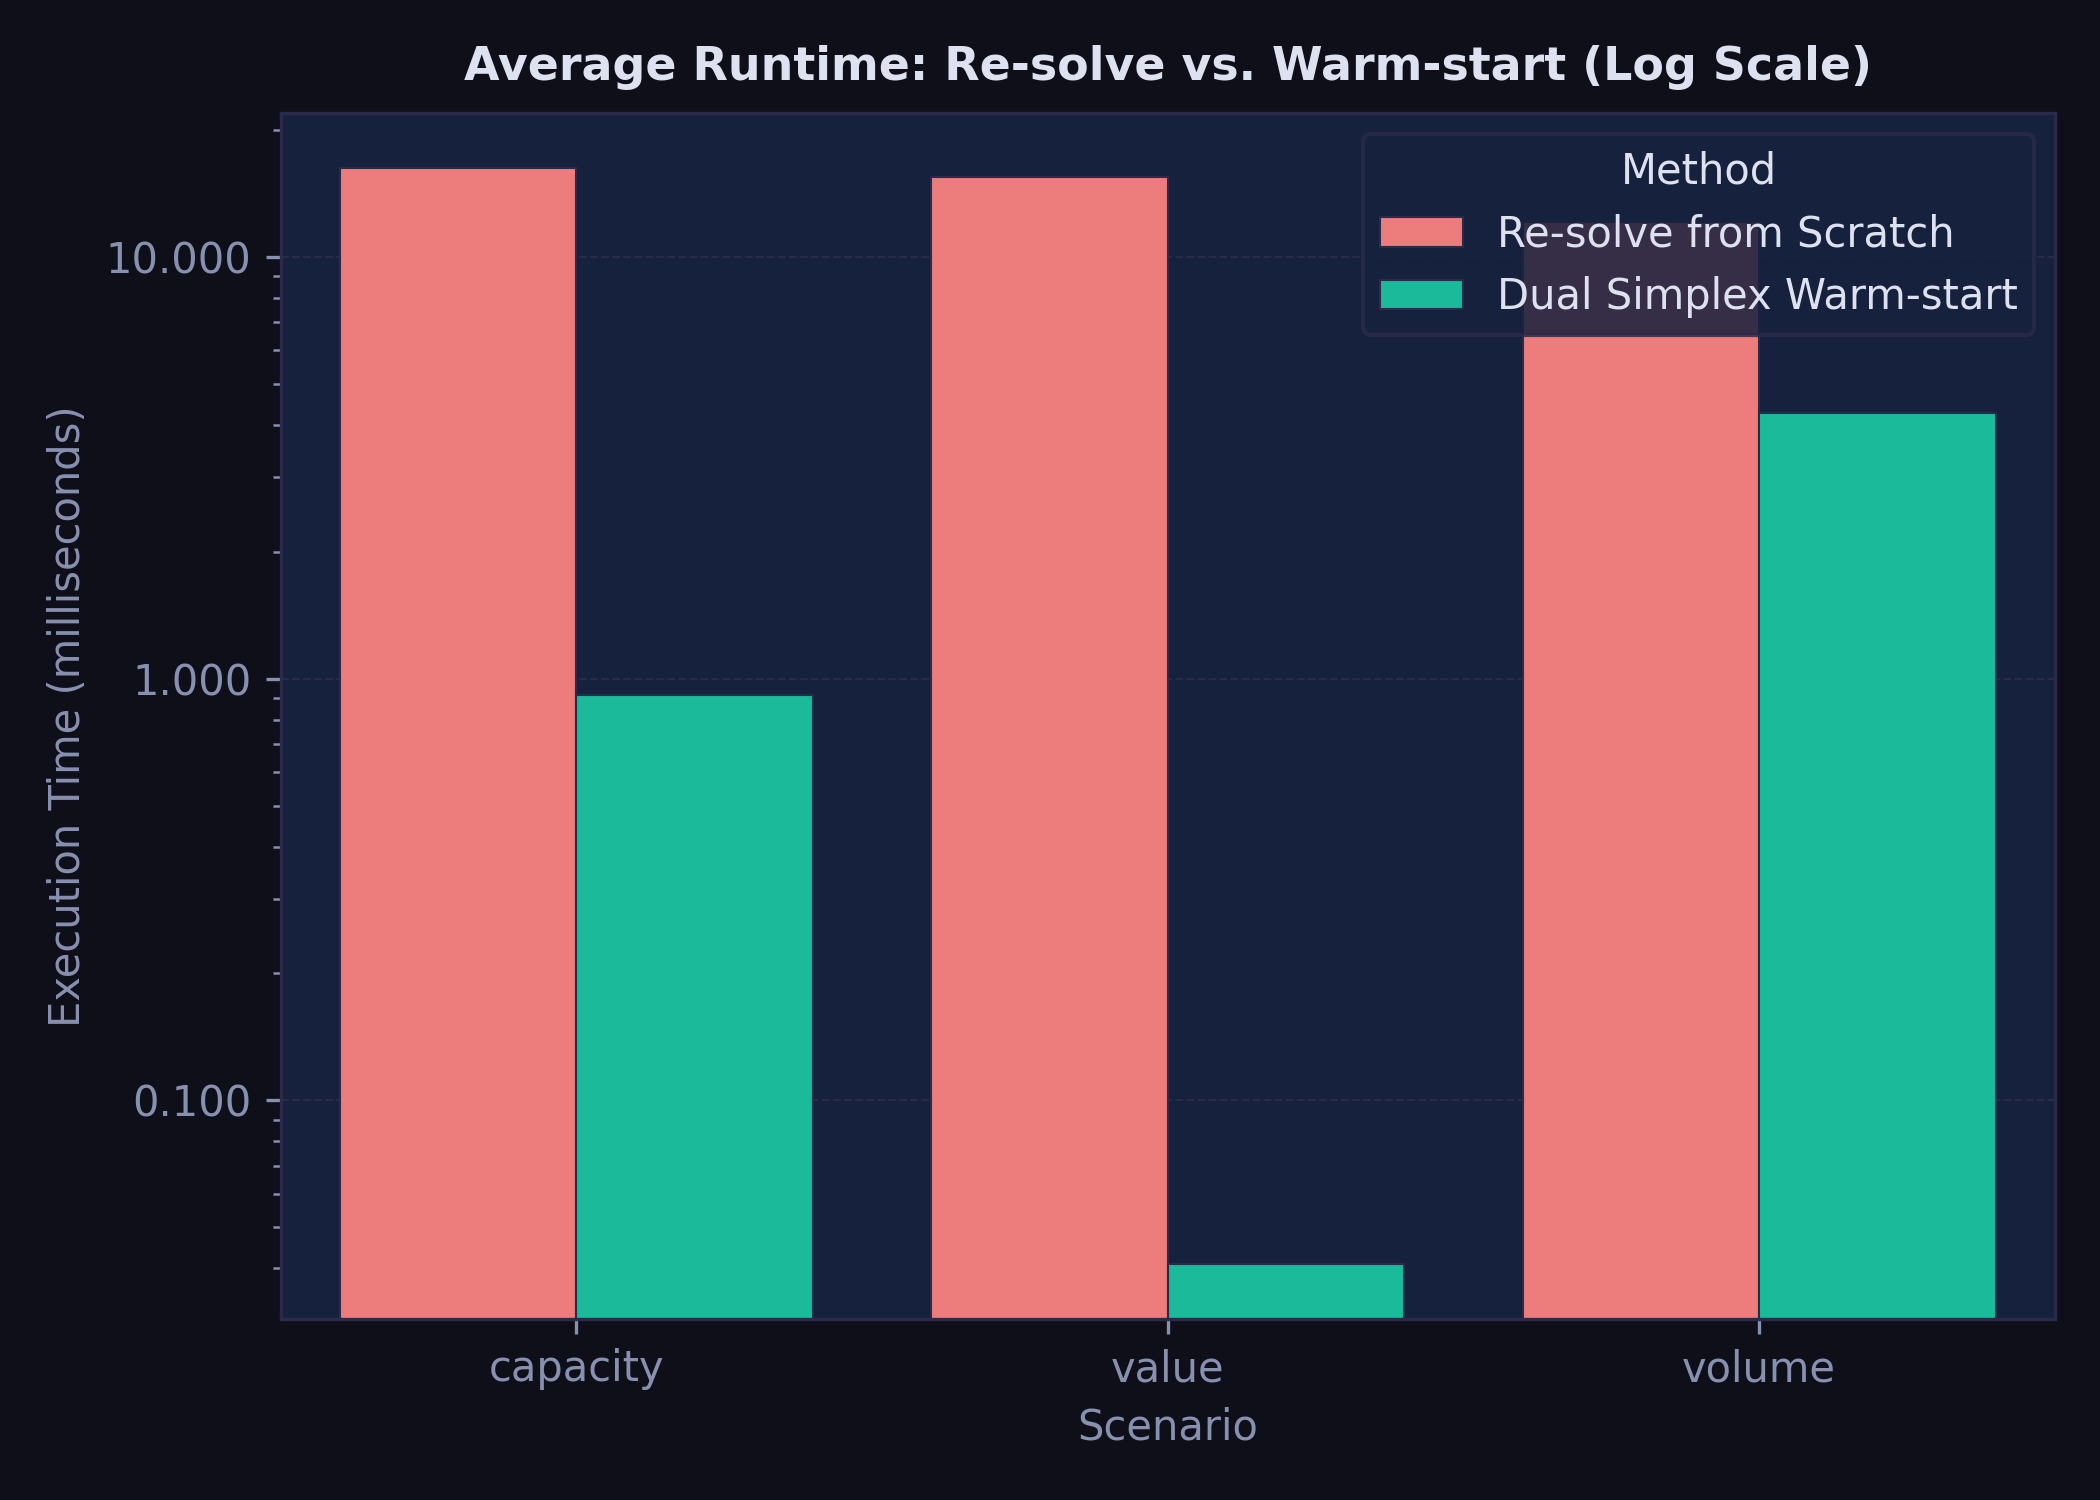
\includegraphics[width=\textwidth]{image/sensitivity/runtime_comparison.png}
                \caption{Thời gian chạy trung bình (ms, log scale).}
            \end{figure}
        \end{column}
        \begin{column}{0.5\textwidth}
            \begin{figure}[H]
                \centering
                
\includegraphics[width=\textwidth]{image/sensitivity/iterations_comparison.png}
                \caption{Số bước xoay pivot trung bình.}
            \end{figure}
        \end{column}
    \end{columns}
    \vspace{0.2em}
    \small
    \textbf{Hiệu quả gia tốc vượt trội:}
    \begin{itemize}
        \item \textbf{Kịch bản Value:} Tăng tốc **$770,0$ lần** (Warm-start chỉ mất $0,37$ bước xoay pivot so với $57,1$ bước khi giải lại từ đầu).
        \item \textbf{Kịch bản Capacity:} Tăng tốc **$24,2$ lần** (xoay pivot $4,3$ bước so với $60,1$ bước).
        \item \textbf{Kịch bản Volume:} Tăng tốc **$5,6$ lần** (xoay pivot $21,2$ bước so với $48,1$ bước).
    \end{itemize}
\end{frame}

% --- Slide 14: Thảo luận sâu sắc & Bài học thuật toán ---
\begin{frame}{Thảo luận sâu sắc \& Bài học thuật toán}
    \begin{itemize}
        \item \textbf{Trade-off giữa tốc độ và tính tổng quát:}
            \begin{itemize}
                \item \texttt{BranchAndBound} combinatorial cực kỳ nhanh trên Knapsack cơ bản nhờ tận dụng cấu trúc một ràng buộc duy nhất.
                \item Simplex/ILP tổng quát bị chậm do chi phí ma trận và khử Gauss, nhưng cực kỳ mạnh mẽ khi giải bài toán có ràng buộc phức tạp hơn (đa chiều, bài toán liên tục) mà các giải thuật tổ hợp chịu bó tay.
            \end{itemize}
        \item \textbf{Cấu trúc cơ sở (basis) làm bộ nhớ hình học:}
            Cơ sở tối ưu lưu giữ thông tin cấu trúc ma trận của bài toán. Việc bảo toàn cơ sở cũ giúp warm-start giải bài toán biến động động cực nhanh, làm nền tảng cho các cây quyết định quy mô lớn.
        \item \textbf{Giới hạn của DP khi capacity lớn:}
            Quy hoạch động mất ưu thế hoàn toàn so với Simplex khi sức chứa $W$ cực lớn và số biến $n$ vừa phải (đã chứng minh trong kịch bản \texttt{stress} và \texttt{core\_heuristic}).
    \end{itemize}
\end{frame}

% --- Slide 15: Kết luận & Hướng phát triển ---
\begin{frame}{Kết luận \& Hướng phát triển}
    \textbf{Các phát hiện định lượng chính:}
    \begin{itemize}
        \item Khẳng định hiệu quả đột phá của \textbf{Warm-start Đơn hình đối ngẫu} trong phân tích độ nhạy (tăng tốc lên tới hơn $770$ lần).
        \item Chứng minh tính chất tối giản bộ nhớ của Simplex tableau ($< 1$\,MB) so với sự bùng nổ của Quy hoạch động ($88,8$\,MB).
        \item Làm rõ lỗi hội tụ do sai số dấu phẩy động trong Python của Gomory Cut và bottleneck khử Gauss tại các nút của Simplex BnB.
    \end{itemize}
    \vspace{0.3em}
    \textbf{Hướng phát triển tương lai:}
    \begin{itemize}
        \item Triển khai các cấu trúc ma trận đơn hình bằng thư viện Cython/Numba để biên dịch mã máy, tối ưu hóa phép khử Gauss tại các nút.
        \item Mở rộng bộ benchmark sang các bài toán tối ưu hóa đa chiều có ràng buộc phức tạp, nơi quy hoạch tuyến tính (LP) thể hiện ưu thế vượt trội.
    \end{itemize}
\end{frame}

% --- Slide 16: Thank You ---
\begin{frame}
    \begin{center}
        \Huge \textbf{\color{deepblue}{CẢM ƠN THẦY CÔ VÀ CÁC BẠN ĐÃ LẮNG NGHE!}}
        
        \vspace{1.5em}
        \large \textbf{Kho lưu trữ mã nguồn dự án:} \\
        \small \url{https://github.com/thucnc7/KnapsackOptimization.git}
    \end{center}
\end{frame}

\end{document}
